\begin{figure}[H]
    \centering
    \begin{subfigure}{0.9\columnwidth}
        \centering
        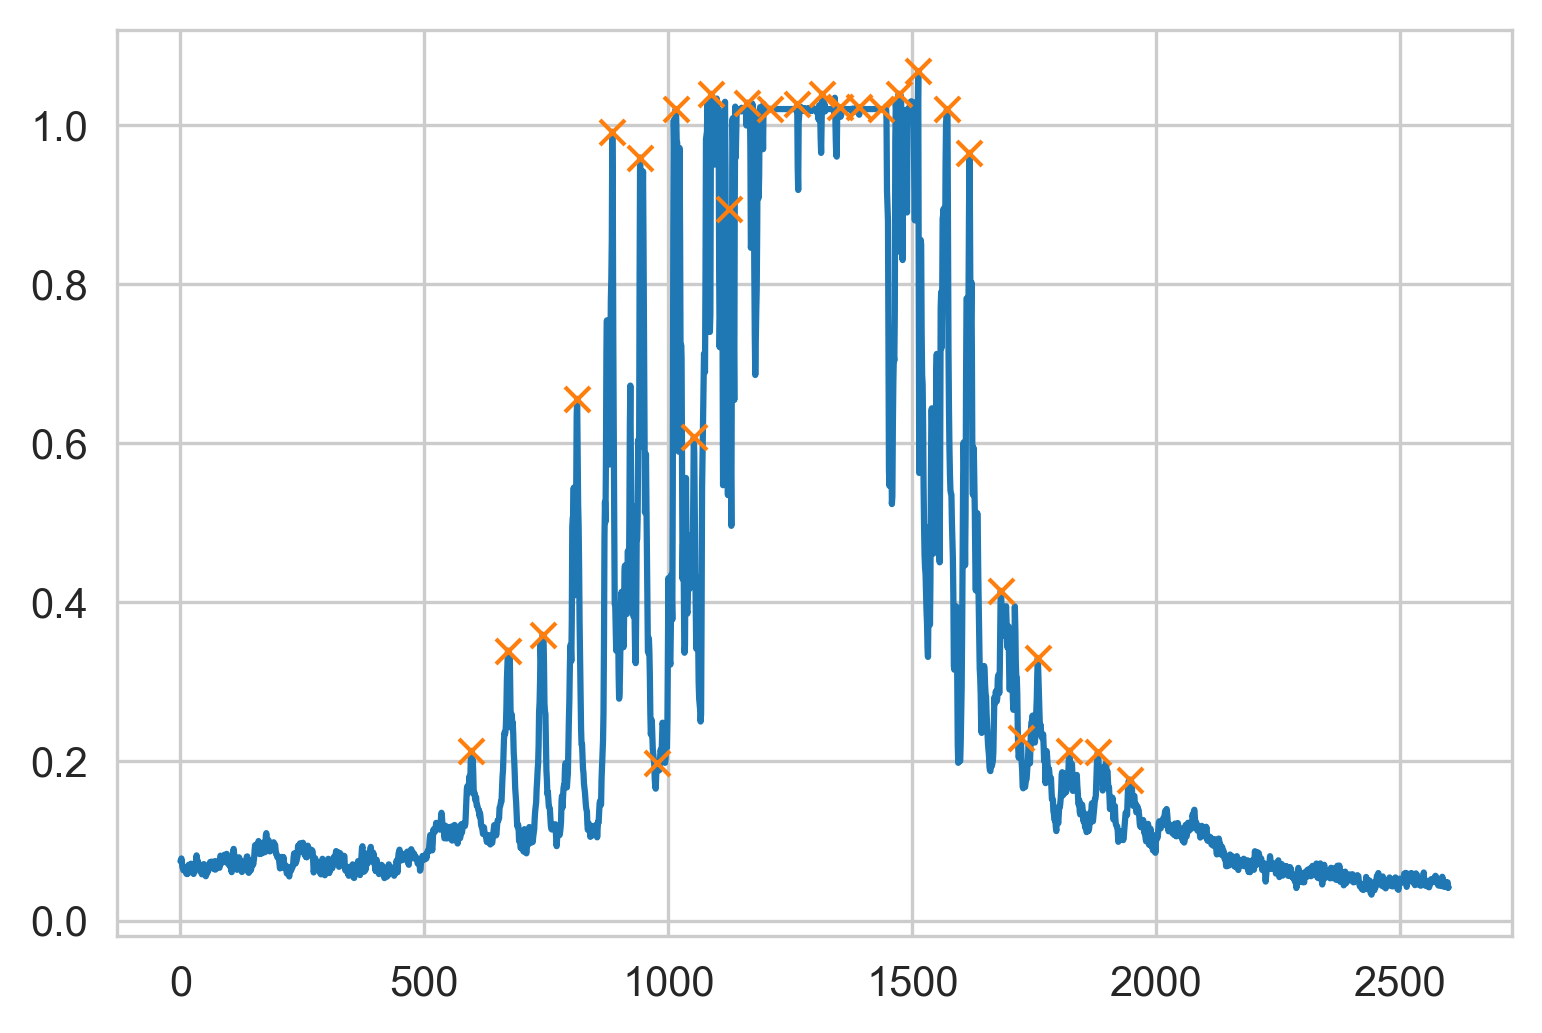
\includegraphics[width=\columnwidth]{figures/X section 1.png} % second figure itself
        \caption{"X" section 1}
        \label{fig:XSection1}
    \end{subfigure}
    \begin{subfigure}{0.9\columnwidth}
        \centering
        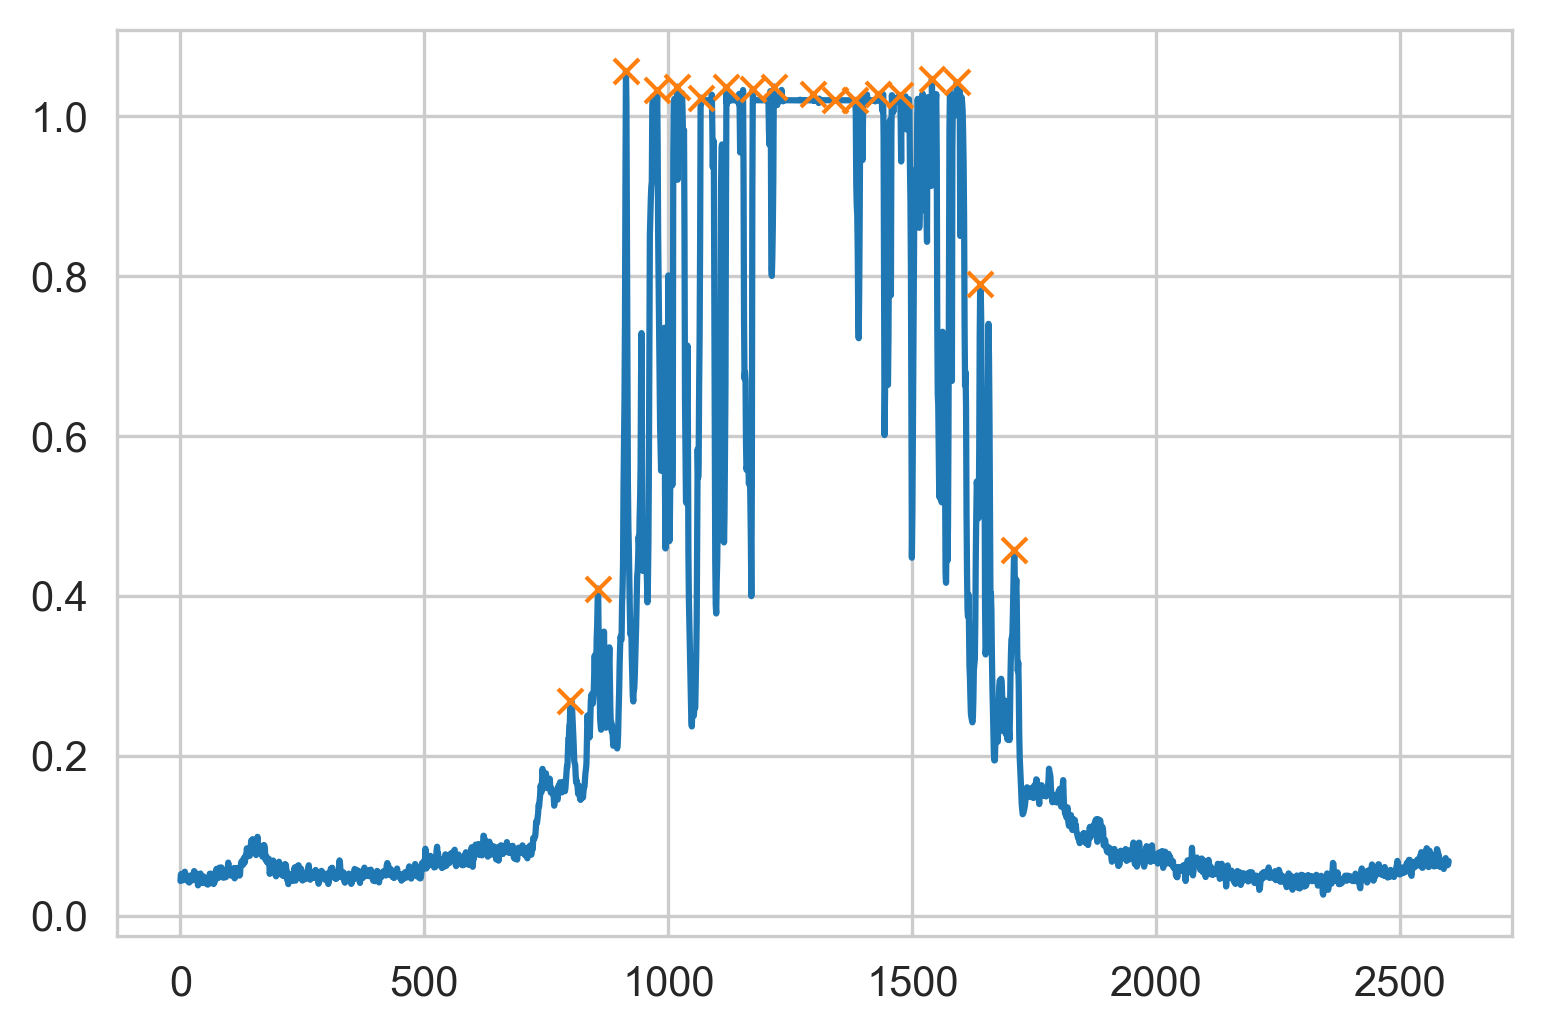
\includegraphics[width=\columnwidth]{figures/X section 2.png}
        \caption{"X" section 2}
        \label{fig:XSection2}
    \end{subfigure}
    \caption{Distances between local maxima along the "X" sections}
    \label{fig:X Sections}
\end{figure}